%% LyX 2.0.6 created this file.  For more info, see http://www.lyx.org/.
%% Do not edit unless you really know what you are doing.
\documentclass{article}\usepackage[]{graphicx}\usepackage[]{color}
%% maxwidth is the original width if it is less than linewidth
%% otherwise use linewidth (to make sure the graphics do not exceed the margin)
\makeatletter
\def\maxwidth{ %
  \ifdim\Gin@nat@width>\linewidth
    \linewidth
  \else
    \Gin@nat@width
  \fi
}
\makeatother

\definecolor{fgcolor}{rgb}{0.345, 0.345, 0.345}
\newcommand{\hlnum}[1]{\textcolor[rgb]{0.686,0.059,0.569}{#1}}%
\newcommand{\hlstr}[1]{\textcolor[rgb]{0.192,0.494,0.8}{#1}}%
\newcommand{\hlcom}[1]{\textcolor[rgb]{0.678,0.584,0.686}{\textit{#1}}}%
\newcommand{\hlopt}[1]{\textcolor[rgb]{0,0,0}{#1}}%
\newcommand{\hlstd}[1]{\textcolor[rgb]{0.345,0.345,0.345}{#1}}%
\newcommand{\hlkwa}[1]{\textcolor[rgb]{0.161,0.373,0.58}{\textbf{#1}}}%
\newcommand{\hlkwb}[1]{\textcolor[rgb]{0.69,0.353,0.396}{#1}}%
\newcommand{\hlkwc}[1]{\textcolor[rgb]{0.333,0.667,0.333}{#1}}%
\newcommand{\hlkwd}[1]{\textcolor[rgb]{0.737,0.353,0.396}{\textbf{#1}}}%

\usepackage{framed}
\makeatletter
\newenvironment{kframe}{%
 \def\at@end@of@kframe{}%
 \ifinner\ifhmode%
  \def\at@end@of@kframe{\end{minipage}}%
  \begin{minipage}{\columnwidth}%
 \fi\fi%
 \def\FrameCommand##1{\hskip\@totalleftmargin \hskip-\fboxsep
 \colorbox{shadecolor}{##1}\hskip-\fboxsep
     % There is no \\@totalrightmargin, so:
     \hskip-\linewidth \hskip-\@totalleftmargin \hskip\columnwidth}%
 \MakeFramed {\advance\hsize-\width
   \@totalleftmargin\z@ \linewidth\hsize
   \@setminipage}}%
 {\par\unskip\endMakeFramed%
 \at@end@of@kframe}
\makeatother

\definecolor{shadecolor}{rgb}{.97, .97, .97}
\definecolor{messagecolor}{rgb}{0, 0, 0}
\definecolor{warningcolor}{rgb}{1, 0, 1}
\definecolor{errorcolor}{rgb}{1, 0, 0}
\newenvironment{knitrout}{}{} % an empty environment to be redefined in TeX

\usepackage{alltt}

\usepackage[sc]{mathpazo}
\usepackage[T1]{fontenc}
\usepackage{geometry}
\usepackage{url}
\geometry{verbose,tmargin=2.5cm,bmargin=2.5cm,lmargin=2.5cm,rmargin=2.5cm}
\setcounter{secnumdepth}{2}
\setcounter{tocdepth}{2}
%\lstset{breaklines=true} % break long lines
\usepackage{url}
\usepackage[unicode=true,pdfusetitle,
 bookmarks=true,bookmarksnumbered=true,bookmarksopen=true,bookmarksopenlevel=2,
  breaklinks=false,pdfborder={0 0 1},backref=false,colorlinks=false]
   {hyperref}
   \hypersetup{
    pdfstartview={XYZ null null 1}}
    \usepackage{breakurl}
\IfFileExists{upquote.sty}{\usepackage{upquote}}{}
    \begin{document}
%\SweaveOpts{concordance=TRUE}

\title{Massifquant Parameter Exploration}
\author{Christopher Conley}

\maketitle
\tableofcontents




\section{Introduction}

Often the default parameters of algorithms for isotope trace (IT) detection can be improved upon for each new data set analyzed. In many multi-parameter algorithms, interest in parameter optimization almost always exceeds patience to do a thorough investigation. A thorough optimization may require hundreds of parameter settings accompanied with (i) an annotation of true IT on a very small subset of the data and (ii) a very clear criteria of evaluation (e.g. f-score). Most analysts cannot afford time to actually conduct this rigorous optimization because it is simply not the end goal. 

By understanding where parameters may be improved and algorithmic tendencies, a practical and efficient optimization is attainable. Massifquant is prone to reporting too many false positives, especially at lower intensities. So simple filters of minimum intensity and length for each IT can eliminate many of these at little cost of true positives with the appropriate tools. \textbf{The tools \& strategy presented here are very intuitive and generally may be applied to other IT detection algorithms like centWave and matchedFilter (with varying success).}

\section{Software \& MOUSE Data Input}

The analysis needs the XCMS software suite to be installed from bioconductor. For further instruction see \url{http://bioconductor.org/packages/release/bioc/html/xcms.html}. The package \emph{xtable} is a nice utility for displaying tables in dynamically generated documents. The \emph{signal} package is useful for doing Savitsky-Golay smoothing to visualize ITs. The \emph{pdist} package efficiently computes the pairwise euclidean distance between two matrices containing different ITs stored in m/z and time coordinates. 

\begin{knitrout}
\definecolor{shadecolor}{rgb}{0.969, 0.969, 0.969}\color{fgcolor}\begin{kframe}
\begin{alltt}
\hlkwd{library}\hlstd{(xcms)}  \hlcom{#massifquant (make sure mzR and Rcpp are under same version build)}
\hlkwd{library}\hlstd{(xtable)}  \hlcom{#latex table generation}
\hlkwd{library}\hlstd{(signal)}  \hlcom{#savitsky-golay filtering}
\hlkwd{library}\hlstd{(pdist)}  \hlcom{#euclidean distance between two matrices }
\end{alltt}
\end{kframe}
\end{knitrout}


There are two ways one may access the MOUSE subsample data files. The easiest is to simply clone the \emph{optimize-it} repository on GitHub (see \url{https://github.com/topherconley/optimize-it}. Alternativly, one may download the MOUSE subsample from the Brigham Young University Scholars' Archive (see \url{http://hdl.lib.byu.edu/1877/3232}). The Scholars' Archive includes  annotation information for those interested.  We illustrate the first option below, while the second is commented out.  It is important to note that this is merely a subset of the original sample. The exact provenance of the sample is detailed in the Massifquant publication. This highly complex sample is good for illustrating optimization because the behavior of the parameters has been well characterized. Hence, the techniques employed below are well-validated. Once downloaded, unzip the contents to a convenient directory. We import the subsample in mzML format and visually confirm it read the data correctly.

\begin{knitrout}
\definecolor{shadecolor}{rgb}{0.969, 0.969, 0.969}\color{fgcolor}\begin{kframe}
\begin{alltt}
\hlcom{# OPTION 1: GitHub}
\hlstd{file_mouse} \hlkwb{<-} \hlkwd{list.files}\hlstd{(}\hlkwc{path} \hlstd{=} \hlstr{"mouse_data"}\hlstd{,} \hlkwc{pattern} \hlstd{=} \hlstr{"mzML"}\hlstd{,} \hlkwc{full.names} \hlstd{=} \hlnum{TRUE}\hlstd{)}
\hlcom{# OPTION 2: scholars' archive archive_path <- 'mouse_annot_complete/dataSourceFile/'}
\hlcom{# file_mouse <- list.files(path = archive_path, pattern = 'mzML', full.names = TRUE)}
\hlstd{data_mouse} \hlkwb{<-} \hlkwd{xcmsRaw}\hlstd{(}\hlkwc{filename} \hlstd{= file_mouse)}
\hlkwd{image}\hlstd{(data_mouse)}
\end{alltt}
\end{kframe}

{\centering 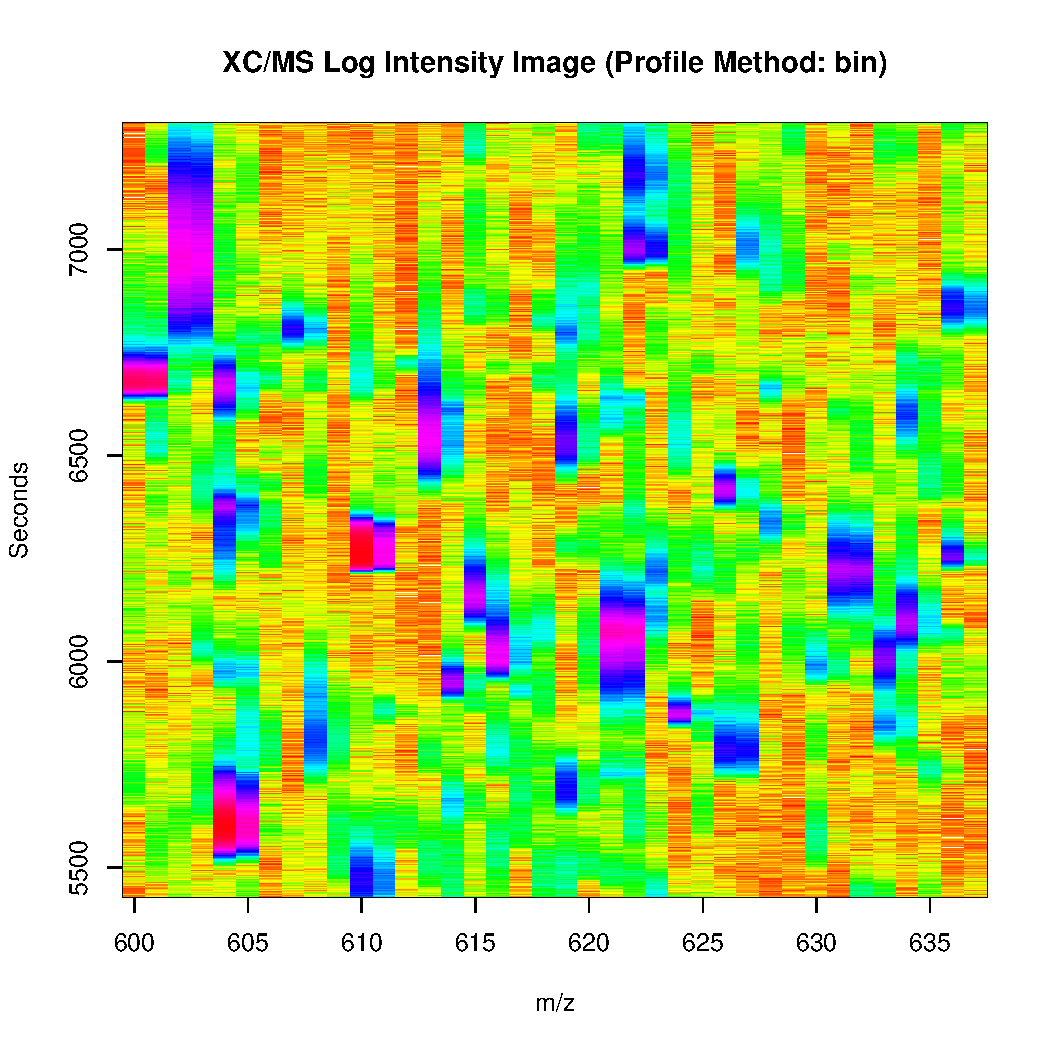
\includegraphics[width=4in,height=4in]{figs/mouse-image} 

}



\end{knitrout}


From this simplified rendering of the MOUSE subsample, one can see general locations of very large ITs.

\section{Simple Filters}

Simple filters are those that post-process the ITs detected by Massifquant's trackers. Minimum length and minimum of the maximum intensity are good examples. With these types of filters, its effective to choose parameters that will tend to report more false positives and then raise the stringency standard as needed. For instance, one might choose low minimum IT intensity and length thresholds. 

% latex table generated in R 3.0.2 by xtable 1.7-3 package
% Mon Mar 31 14:46:59 2014
\begin{table}[ht]
\centering
\begin{tabular}{rrrrrr}
  \hline
 & prefilter[2] & peakwidth[1] & ppm & criticalValue & consecMissedLimit \\ 
  \hline
1 & 65000.00 & 15.00 & 25.00 & 1.50 & 2.00 \\ 
   \hline
\end{tabular}
\caption{First Pass Leniency} 
\end{table}



Next run Massifquant under these parameters inducing high false positives and with paramter values that are intentionally not exactly the same as what was found to be best in the formal evaluation of MOUSE. It is valuable to see how visually-driven optimization methods presented in this analysis compare with a formulaic f-score approach. 

\begin{knitrout}
\definecolor{shadecolor}{rgb}{0.969, 0.969, 0.969}\color{fgcolor}\begin{kframe}
\begin{alltt}
\hlstd{ixs} \hlkwb{<-} \hlkwd{xcmsSet}\hlstd{(}\hlkwc{files} \hlstd{= file_mouse,} \hlkwc{method} \hlstd{=} \hlstr{"massifquant"}\hlstd{,} \hlkwc{prefilter} \hlstd{=} \hlkwd{c}\hlstd{(}\hlnum{1}\hlstd{,} \hlnum{65000}\hlstd{),} \hlkwc{peakwidth} \hlstd{=} \hlkwd{c}\hlstd{(}\hlnum{15}\hlstd{,}
    \hlnum{100}\hlstd{),} \hlkwc{ppm} \hlstd{=} \hlnum{25}\hlstd{,} \hlkwc{criticalValue} \hlstd{=} \hlnum{1.5}\hlstd{,} \hlkwc{consecMissedLimit} \hlstd{=} \hlnum{2}\hlstd{,} \hlkwc{withWave} \hlstd{=} \hlnum{0}\hlstd{)}
\end{alltt}
\end{kframe}
\end{knitrout}


\subsection{Minimum Intensity Filter}

The reported IT of this first pass are then subjected to increasing intensity thresholds to see the elimination effect each threshold has on reported IT. As seen in the figure below, the chosen intensity thresholds have a non-negligle effect on the number of peaks reported in the algorithm.

\begin{knitrout}
\definecolor{shadecolor}{rgb}{0.969, 0.969, 0.969}\color{fgcolor}

{\centering 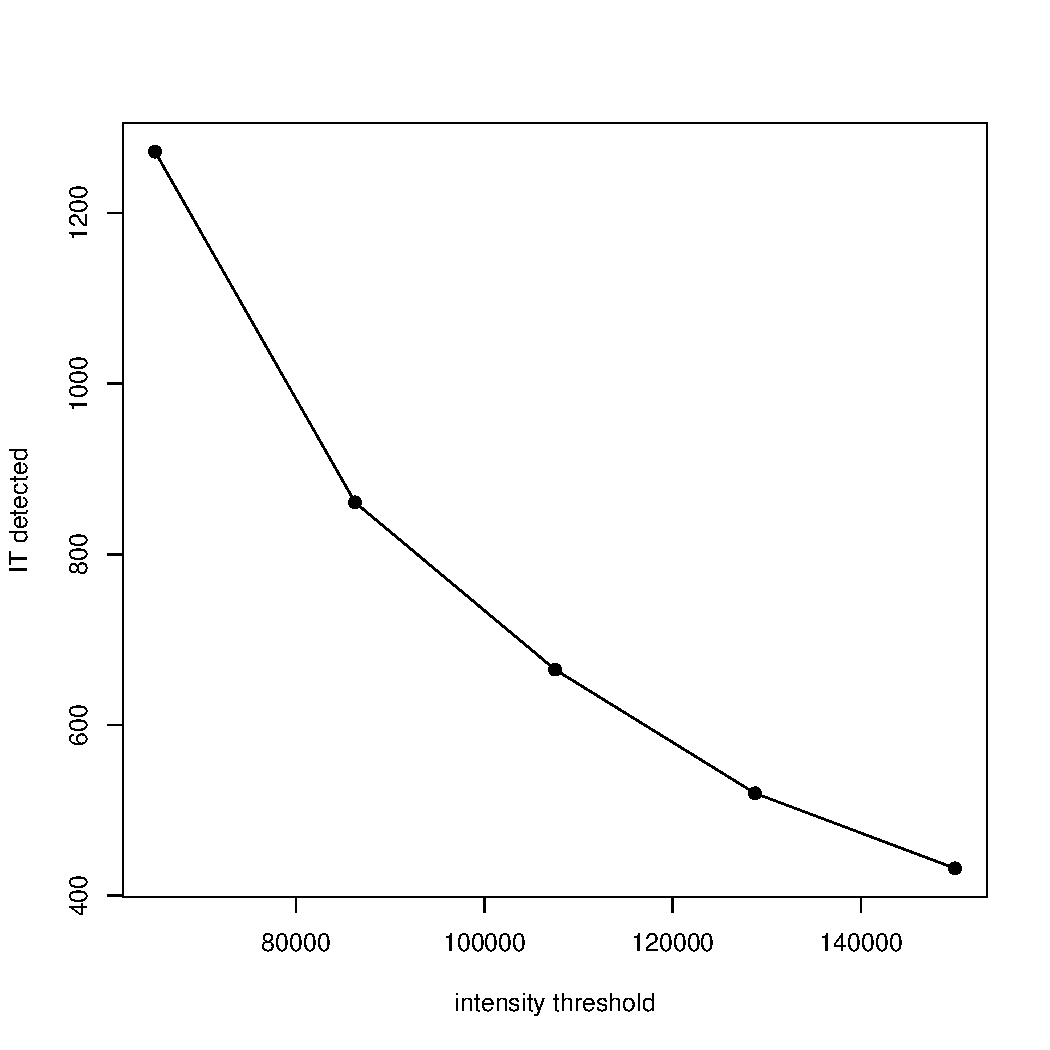
\includegraphics[width=4in,height=4in]{figs/numpeaks-intensity} 

}



\end{knitrout}


\subsection{Relaxed IT Set Contribution (RISC)}

For any two intensity thresholds generating IT sets $A,B$, we can investigate the effect of the more stringent threshold that generated the set $B$. Specifically, we can evaluate the importance of the IT set $A \setminus B = \{x \in A : x \notin B \}$, denoted as the relaxed IT set contribution (RISC). Often, for simple post-processing parameters like intensity or length, we have a special RISC, where $B \subset A$. Under this subset condition, if the RISC contains important features, then we should keep the more relaxed threshold generating $A$. Plotting and saving arbitrary IT sets (e.g. RISC) to file allows for a relatively quick determination of how to choose between two thresholds, which is what the following ``plot IT set'' function achieves. In cases where there are sufficient centroids, a Savitsky-Golay smoother overlays a solid black line over the spectra.

\begin{knitrout}
\definecolor{shadecolor}{rgb}{0.969, 0.969, 0.969}\color{fgcolor}\begin{kframe}
\begin{alltt}
\hlstd{plot_it_set} \hlkwb{<-} \hlkwa{function}\hlstd{(}\hlkwc{xr}\hlstd{,} \hlkwc{xs}\hlstd{,} \hlkwc{filename} \hlstd{=} \hlkwa{NULL}\hlstd{,} \hlkwc{it_set_idx}\hlstd{) \{}
    \hlstd{write_to_file} \hlkwb{<-} \hlopt{!}\hlkwd{is.null}\hlstd{(filename)}
    \hlkwa{if} \hlstd{(write_to_file)}
        \hlkwd{pdf}\hlstd{(filename,} \hlkwc{height} \hlstd{=} \hlnum{8}\hlstd{,} \hlkwc{width} \hlstd{=} \hlnum{8}\hlstd{,} \hlkwc{onefile} \hlstd{=} \hlnum{TRUE}\hlstd{)}
    \hlstd{ncentroids} \hlkwb{<-} \hlkwd{vector}\hlstd{(}\hlkwc{mode} \hlstd{=} \hlstr{"integer"}\hlstd{,} \hlkwc{length} \hlstd{=} \hlkwd{length}\hlstd{(it_set_idx))}
    \hlstd{cnt} \hlkwb{<-} \hlnum{1}
    \hlkwa{for} \hlstd{(idx} \hlkwa{in} \hlstd{it_set_idx) \{}
        \hlkwd{par}\hlstd{(}\hlkwc{mfrow} \hlstd{=} \hlkwd{c}\hlstd{(}\hlnum{2}\hlstd{,} \hlnum{1}\hlstd{))}
        \hlstd{mzr} \hlkwb{<-} \hlstd{xs}\hlopt{@}\hlkwc{peaks}\hlstd{[idx,} \hlkwd{c}\hlstd{(}\hlstr{"mzmin"}\hlstd{,} \hlstr{"mzmax"}\hlstd{)]}
        \hlstd{rtr} \hlkwb{<-} \hlstd{xs}\hlopt{@}\hlkwc{peaks}\hlstd{[idx,} \hlkwd{c}\hlstd{(}\hlstr{"rtmin"}\hlstd{,} \hlstr{"rtmax"}\hlstd{)]}
        \hlstd{it_data} \hlkwb{<-} \hlkwd{plotRaw}\hlstd{(xr, mzr, rtr,} \hlkwc{title} \hlstd{=} \hlkwd{paste}\hlstd{(}\hlstr{"IT Index:"}\hlstd{, idx))}
        \hlstd{ymax} \hlkwb{<-} \hlkwd{max}\hlstd{(it_data[,} \hlstr{"intensity"}\hlstd{])}
        \hlstd{colorlut} \hlkwb{<-} \hlkwd{terrain.colors}\hlstd{(}\hlnum{16}\hlstd{)}
        \hlstd{col} \hlkwb{<-} \hlstd{colorlut[it_data[,} \hlstr{"intensity"}\hlstd{]}\hlopt{/}\hlstd{ymax} \hlopt{*} \hlnum{15} \hlopt{+} \hlnum{1}\hlstd{]}
        \hlkwd{plot}\hlstd{(it_data[,} \hlnum{1}\hlstd{], it_data[,} \hlnum{3}\hlstd{],} \hlkwc{pch} \hlstd{=} \hlnum{19}\hlstd{,} \hlkwc{type} \hlstd{=} \hlstr{"h"}\hlstd{,} \hlkwc{col} \hlstd{= col,} \hlkwc{xlab} \hlstd{=} \hlstr{"Seconds"}\hlstd{,}
            \hlkwc{ylab} \hlstd{=} \hlstr{"Intensity"}\hlstd{)}
        \hlstd{ncentroids[cnt]} \hlkwb{<-} \hlkwd{nrow}\hlstd{(it_data)}
        \hlkwa{if} \hlstd{(ncentroids[cnt]} \hlopt{>} \hlnum{30}\hlstd{) \{}
            \hlstd{nwindow} \hlkwb{<-} \hlkwd{round}\hlstd{(ncentroids[cnt]}\hlopt{/}\hlnum{3}\hlstd{)}
            \hlkwa{if} \hlstd{(nwindow}\hlopt\hlnum{2} \hlopt{==} \hlnum{0}\hlstd{)}
                \hlstd{nwindow} \hlkwb{<-} \hlstd{nwindow} \hlopt{-} \hlnum{1}
            \hlstd{sg} \hlkwb{<-} \hlkwd{sgolay}\hlstd{(}\hlkwc{p} \hlstd{=} \hlnum{2}\hlstd{,} \hlkwc{n} \hlstd{= nwindow,} \hlkwc{m} \hlstd{=} \hlnum{0}\hlstd{,} \hlkwc{ts} \hlstd{=} \hlkwd{mean}\hlstd{(}\hlkwd{diff}\hlstd{(it_data[,} \hlstr{"time"}\hlstd{])))}
            \hlstd{ysg} \hlkwb{<-} \hlkwd{filter}\hlstd{(sg,} \hlkwc{x} \hlstd{= it_data[,} \hlstr{"intensity"}\hlstd{])}
            \hlkwd{lines}\hlstd{(}\hlkwc{x} \hlstd{= it_data[,} \hlstr{"time"}\hlstd{],} \hlkwc{y} \hlstd{= ysg,} \hlkwc{lwd} \hlstd{=} \hlnum{3}\hlstd{,} \hlkwc{col} \hlstd{=} \hlstr{"black"}\hlstd{)}
        \hlstd{\}}
        \hlstd{cnt} \hlkwb{<-} \hlstd{cnt} \hlopt{+} \hlnum{1}
    \hlstd{\}}
    \hlkwa{if} \hlstd{(write_to_file)}
        \hlkwd{dev.off}\hlstd{()}
    \hlkwd{return}\hlstd{(ncentroids)}
\hlstd{\}}
\end{alltt}
\end{kframe}
\end{knitrout}


For example, with the five thresholds chosen we will investigate adjacent threshold contributions through the sets $\{ RISC_{i, i + 1} : i = 1,2,3,4 \}$. Below we plot the RISC and save the results to a separate file because the size of each set is respectively (411, 196, 145, 88). 
\begin{knitrout}
\definecolor{shadecolor}{rgb}{0.969, 0.969, 0.969}\color{fgcolor}\begin{kframe}
\begin{alltt}
\hlstd{iRISC} \hlkwb{<-} \hlkwd{sapply}\hlstd{(}\hlnum{1}\hlopt{:}\hlstd{(}\hlkwd{length}\hlstd{(idetect)} \hlopt{-} \hlnum{1}\hlstd{),} \hlkwa{function}\hlstd{(}\hlkwc{j}\hlstd{) \{}
    \hlstd{f} \hlkwb{<-} \hlkwd{paste}\hlstd{(}\hlstr{"figs/iRISC"}\hlstd{, j, j} \hlopt{+} \hlnum{1}\hlstd{,} \hlstr{".pdf"}\hlstd{,} \hlkwc{sep} \hlstd{=} \hlstr{"-"}\hlstd{)}
    \hlstd{idx} \hlkwb{<-} \hlkwd{setdiff}\hlstd{(idetect[[j]], idetect[[j} \hlopt{+} \hlnum{1}\hlstd{]])}
    \hlkwd{plot_it_set}\hlstd{(}\hlkwc{xr} \hlstd{= data_mouse,} \hlkwc{xs} \hlstd{= ixs,} \hlkwc{filename} \hlstd{= f,} \hlkwc{it_set_idx} \hlstd{= idx)}
\hlstd{\})}
\end{alltt}
\end{kframe}
\end{knitrout}


Visual inspection shows $RISC_{1,2},RISC_{2,3}$ are almost pure noise, meaning the first two thresholds are too lenient. For example, the figure below shows a false postive IT with very low intensity.
\begin{knitrout}
\definecolor{shadecolor}{rgb}{0.969, 0.969, 0.969}\color{fgcolor}

{\centering 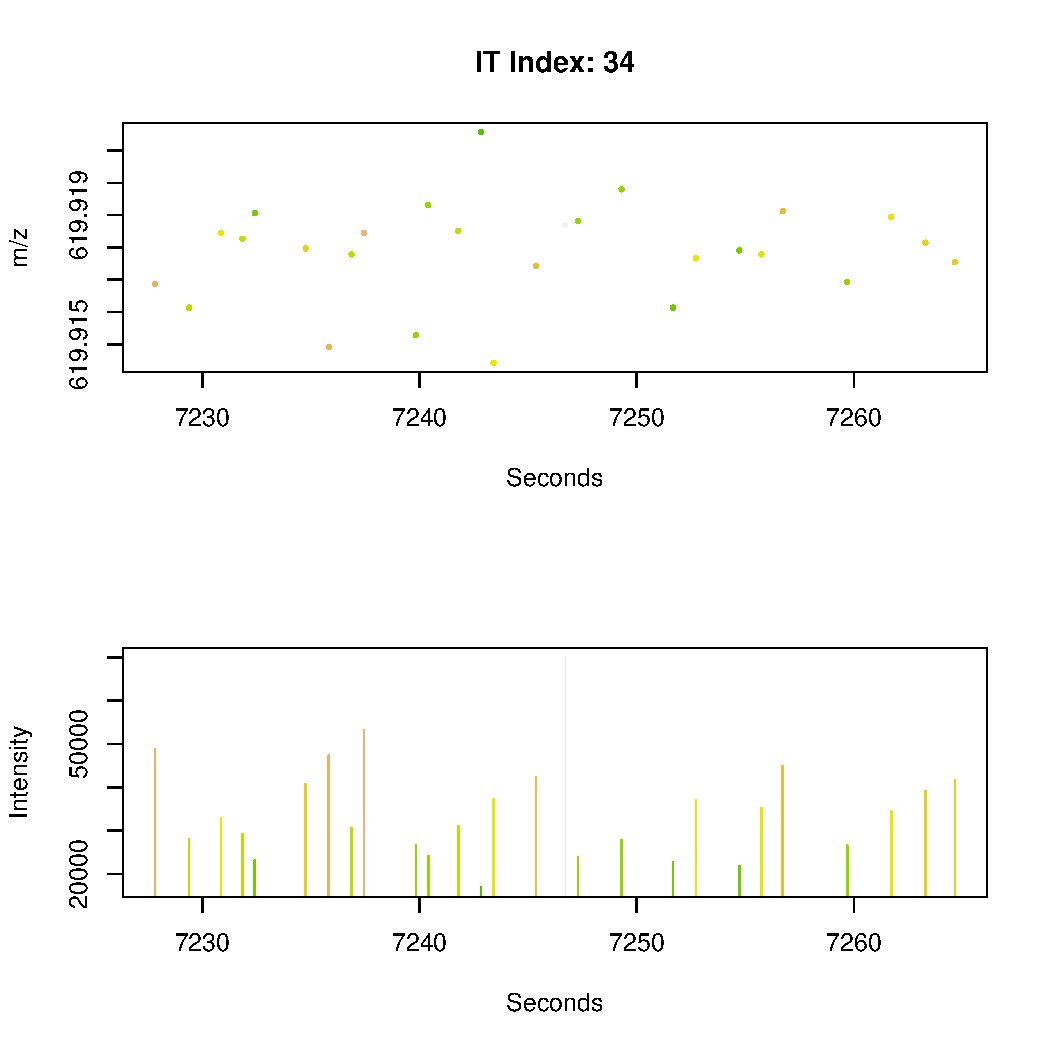
\includegraphics[width=5in,height=5in]{figs/noise-IT-low-intensity} 

}



\end{knitrout}


$RISC_{3,4}$ shows some legitimate ITs that will be lost if we strictly use the 3rd threshold. $RISC_{4,5}$ has about 50\% potential true positives (just eye-balling feature shape). Globally this is unacceptable, but remember, most of the false positives come from the low intensity features, which is the case in this set. Depending on the project's aims, the analyst might vary the the tolerance of low-intensity false positives. The next figure comes from the $RISC_{4,5}$ to justify using the 4th threshold instead of the 5th. Further, the manual annotation recorded 589 true ITs, which is in the same neighborhood as the number of features (520) under the 4th threshold. Of course, one can further tune these filter parameters, but for the purposes of this exercise we are satisfied. 
\begin{knitrout}
\definecolor{shadecolor}{rgb}{0.969, 0.969, 0.969}\color{fgcolor}

{\centering 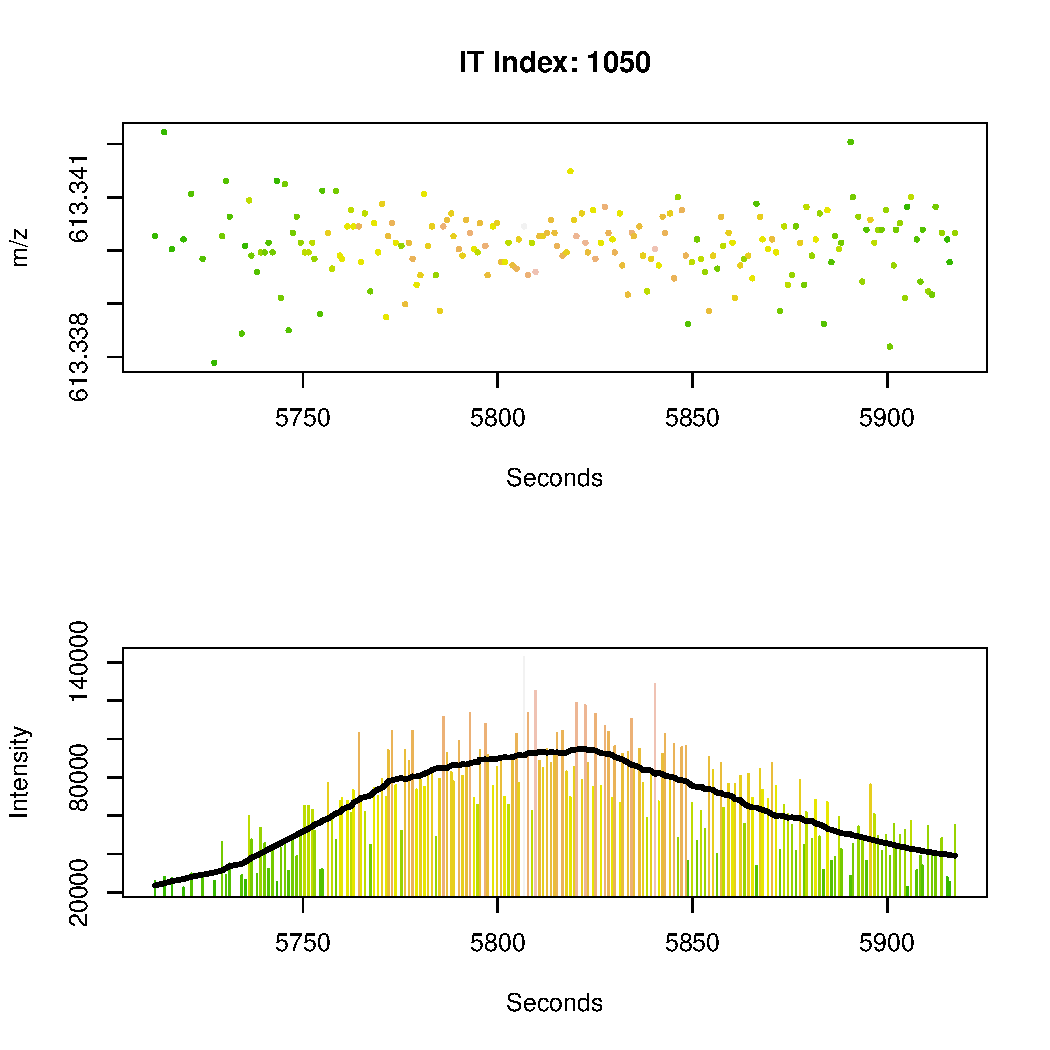
\includegraphics[width=5in,height=5in]{figs/bonafide-IT-low-intensity} 

}



\end{knitrout}


% latex table generated in R 3.0.2 by xtable 1.7-3 package
% Mon Mar 31 14:47:17 2014
\begin{table}[ht]
\centering
\begin{tabular}{rrrrrr}
  \hline
 & prefilter[2] & peakwidth[1] & ppm & criticalValue & consecMissedLimit \\ 
  \hline
1 & 65000.00 & 15.00 & 25.00 & 1.50 & 2.00 \\ 
  2 & 128750.00 & 15.00 & 25.00 & 1.50 & 2.00 \\ 
   \hline
\end{tabular}
\caption{Second Parameter Pass} 
\end{table}



\subsection{Minimum Length Filter}
Now we can potentially improve upon the filter for the minimum length in the same fashion applied to the minimum intensity. Run Massifquant with the updated min intensity setting (prefilter[2]) and the result is slightly different than 520. The reason is that the segmentation correction was applied under a more stringent intensity than the original parameter setting. The difference should not be significant. 

\begin{knitrout}
\definecolor{shadecolor}{rgb}{0.969, 0.969, 0.969}\color{fgcolor}\begin{kframe}
\begin{alltt}
\hlstd{lxs} \hlkwb{<-} \hlkwd{xcmsSet}\hlstd{(}\hlkwc{files} \hlstd{= file_mouse,} \hlkwc{method} \hlstd{=} \hlstr{"massifquant"}\hlstd{,} \hlkwc{prefilter} \hlstd{=} \hlkwd{c}\hlstd{(}\hlnum{1}\hlstd{,} \hlnum{128750}\hlstd{),} \hlkwc{peakwidth} \hlstd{=} \hlkwd{c}\hlstd{(}\hlnum{15}\hlstd{,}
    \hlnum{100}\hlstd{),} \hlkwc{ppm} \hlstd{=} \hlnum{25}\hlstd{,} \hlkwc{criticalValue} \hlstd{=} \hlnum{1.5}\hlstd{,} \hlkwc{consecMissedLimit} \hlstd{=} \hlnum{2}\hlstd{,} \hlkwc{withWave} \hlstd{=} \hlnum{0}\hlstd{)}
\end{alltt}
\end{kframe}
\end{knitrout}


To get the length of each feature, we could simply subtract the retention time minimum from the maximum, but this is slightly inaccurate because of time warping that has not been corrected for. 
\begin{knitrout}
\definecolor{shadecolor}{rgb}{0.969, 0.969, 0.969}\color{fgcolor}\begin{kframe}
\begin{alltt}
\hlstd{lidxs} \hlkwb{<-} \hlkwd{seq_len}\hlstd{(}\hlkwd{nrow}\hlstd{(lxs}\hlopt{@}\hlkwc{peaks}\hlstd{))}
\hlstd{len_lxs} \hlkwb{<-} \hlkwd{plot_it_set}\hlstd{(data_mouse, lxs,} \hlstr{"figs/tmp.pdf"}\hlstd{, lidxs)}
\hlstd{rm_tmpfig} \hlkwb{<-} \hlkwd{system}\hlstd{(}\hlstr{"rm figs/tmp.pdf"}\hlstd{)}
\hlstd{lthreshold} \hlkwb{<-} \hlkwd{seq}\hlstd{(}\hlkwc{from} \hlstd{=} \hlnum{15}\hlstd{,} \hlkwc{to} \hlstd{=} \hlnum{80}\hlstd{,} \hlkwc{by} \hlstd{=} \hlnum{15}\hlstd{)}
\hlstd{ldetect} \hlkwb{<-} \hlkwd{lapply}\hlstd{(lthreshold,} \hlkwa{function}\hlstd{(}\hlkwc{l}\hlstd{)} \hlkwd{which}\hlstd{(len_lxs} \hlopt{>=} \hlstd{l))}
\hlstd{lnumdetect} \hlkwb{<-} \hlkwd{sapply}\hlstd{(ldetect, length)}
\end{alltt}
\end{kframe}
\end{knitrout}


The RISCs are generated under the varying length thresholds.

\begin{knitrout}
\definecolor{shadecolor}{rgb}{0.969, 0.969, 0.969}\color{fgcolor}\begin{kframe}
\begin{alltt}
\hlstd{lenRISC} \hlkwb{<-} \hlkwd{sapply}\hlstd{(}\hlnum{1}\hlopt{:}\hlstd{(}\hlkwd{length}\hlstd{(ldetect)} \hlopt{-} \hlnum{1}\hlstd{),} \hlkwa{function}\hlstd{(}\hlkwc{j}\hlstd{) \{}
    \hlstd{f} \hlkwb{<-} \hlkwd{paste}\hlstd{(}\hlstr{"figs/lenRISC"}\hlstd{, j, j} \hlopt{+} \hlnum{1}\hlstd{,} \hlstr{".pdf"}\hlstd{,} \hlkwc{sep} \hlstd{=} \hlstr{"-"}\hlstd{)}
    \hlstd{idx} \hlkwb{<-} \hlkwd{setdiff}\hlstd{(ldetect[[j]], ldetect[[j} \hlopt{+} \hlnum{1}\hlstd{]])}
    \hlkwd{plot_it_set}\hlstd{(}\hlkwc{xr} \hlstd{= data_mouse,} \hlkwc{xs} \hlstd{= lxs,} \hlkwc{filename} \hlstd{= f,} \hlkwc{it_set_idx} \hlstd{= idx)}
\hlstd{\})}
\end{alltt}
\end{kframe}
\end{knitrout}


For the minimum length filter, it is not until about $RISC_{4,5}$ do we start to see many legitimate features that would be lost if the stringency exceeded the 4th length threshold. Below is a an example of a true postive IT that would be unreported under the 5th length threshold. Losing true positive ITs is the cost of being too stringent.

\begin{knitrout}
\definecolor{shadecolor}{rgb}{0.969, 0.969, 0.969}\color{fgcolor}

{\centering 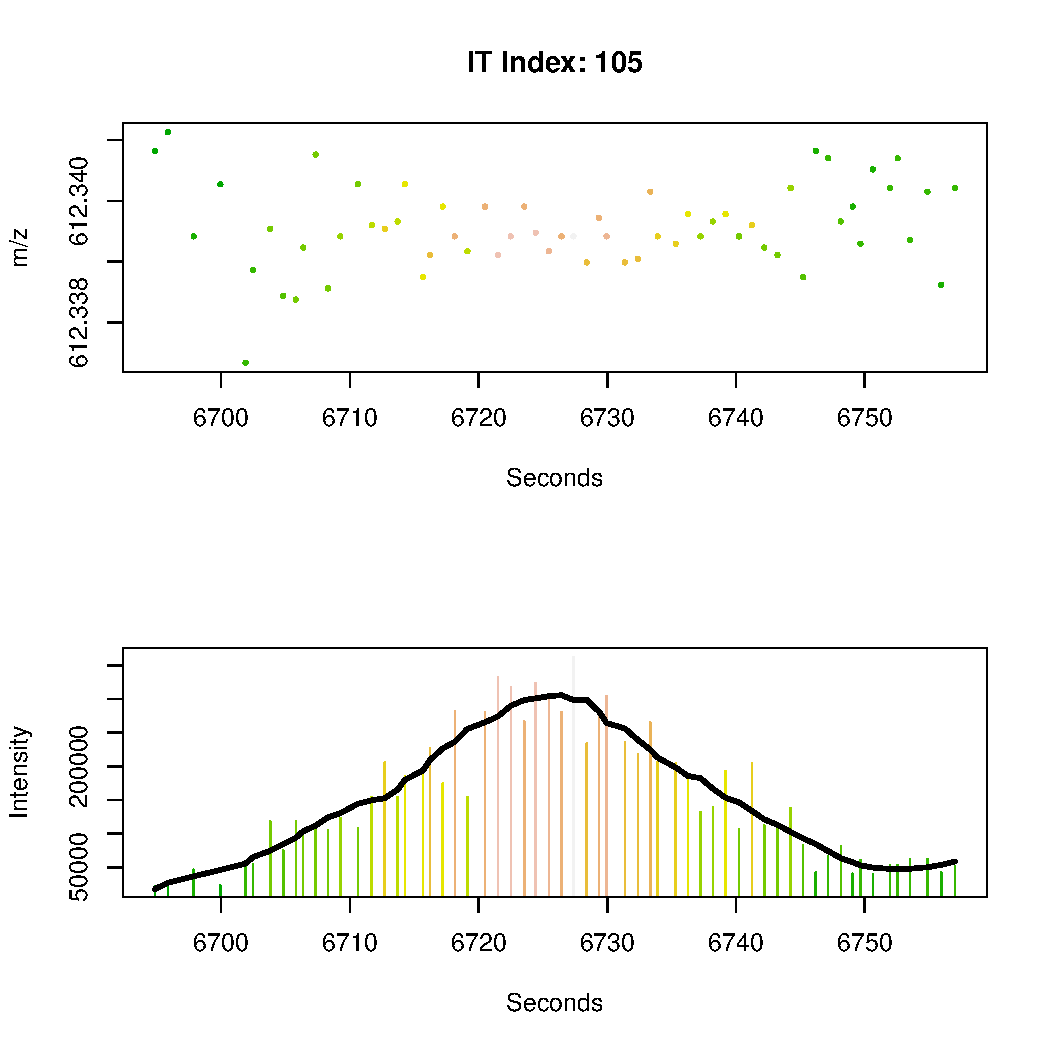
\includegraphics[width=5in,height=5in]{figs/bonafide-IT-lower-length} 

}



\end{knitrout}


The simple RISC filter strategy affords predictable optimization outcomes. The filters eliminate a lot of false positives in the subsample that would likely be encountered on the whole sample. It also happens to preserve many prominent IT. 

\subsection{Comparing visual vs. formula-driven optimization outcomes}

How does a visual RISC optimization strategy compare to a greedy search cross referencing reported ITs to an annotation with precise metrics (e.g. f-score) as presented in the Massifquant publication?  The former is quick and simple, while the latter is time-consuming and more sophisticated. Can the simplicity of exploratory data analysis be justified? Here Massifquant is run once more with the final length and intensity filters and the IT set generated is visually confirmed in the pdf file,``fxs-out-ITs''. The same visualization could be done for the greedy-search optimized parameters. The figure below illustrates a prominent IT from the MOUSE subsample.

\begin{knitrout}
\definecolor{shadecolor}{rgb}{0.969, 0.969, 0.969}\color{fgcolor}\begin{kframe}
\begin{alltt}
\hlstd{fxs} \hlkwb{<-} \hlkwd{xcmsSet}\hlstd{(}\hlkwc{files} \hlstd{= file_mouse,} \hlkwc{method} \hlstd{=} \hlstr{"massifquant"}\hlstd{,} \hlkwc{prefilter} \hlstd{=} \hlkwd{c}\hlstd{(}\hlnum{1}\hlstd{,} \hlnum{128750}\hlstd{),} \hlkwc{peakwidth} \hlstd{=} \hlkwd{c}\hlstd{(}\hlnum{60}\hlstd{,}
    \hlnum{100}\hlstd{),} \hlkwc{ppm} \hlstd{=} \hlnum{25}\hlstd{,} \hlkwc{criticalValue} \hlstd{=} \hlnum{1.5}\hlstd{,} \hlkwc{consecMissedLimit} \hlstd{=} \hlnum{2}\hlstd{,} \hlkwc{withWave} \hlstd{=} \hlnum{0}\hlstd{)}
\hlstd{all_idxs} \hlkwb{<-} \hlkwd{seq_len}\hlstd{(}\hlkwd{nrow}\hlstd{(fxs}\hlopt{@}\hlkwc{peaks}\hlstd{))}
\hlkwd{plot_it_set}\hlstd{(data_mouse, fxs,} \hlstr{"figs/fxs-out-ITs.pdf"}\hlstd{, all_idxs)}
\hlkwd{plot_it_set}\hlstd{(}\hlkwc{xr} \hlstd{= data_mouse,} \hlkwc{xs} \hlstd{= fxs,} \hlkwc{it_set_idx} \hlstd{=} \hlnum{93}\hlstd{)}
\end{alltt}
\end{kframe}

{\centering 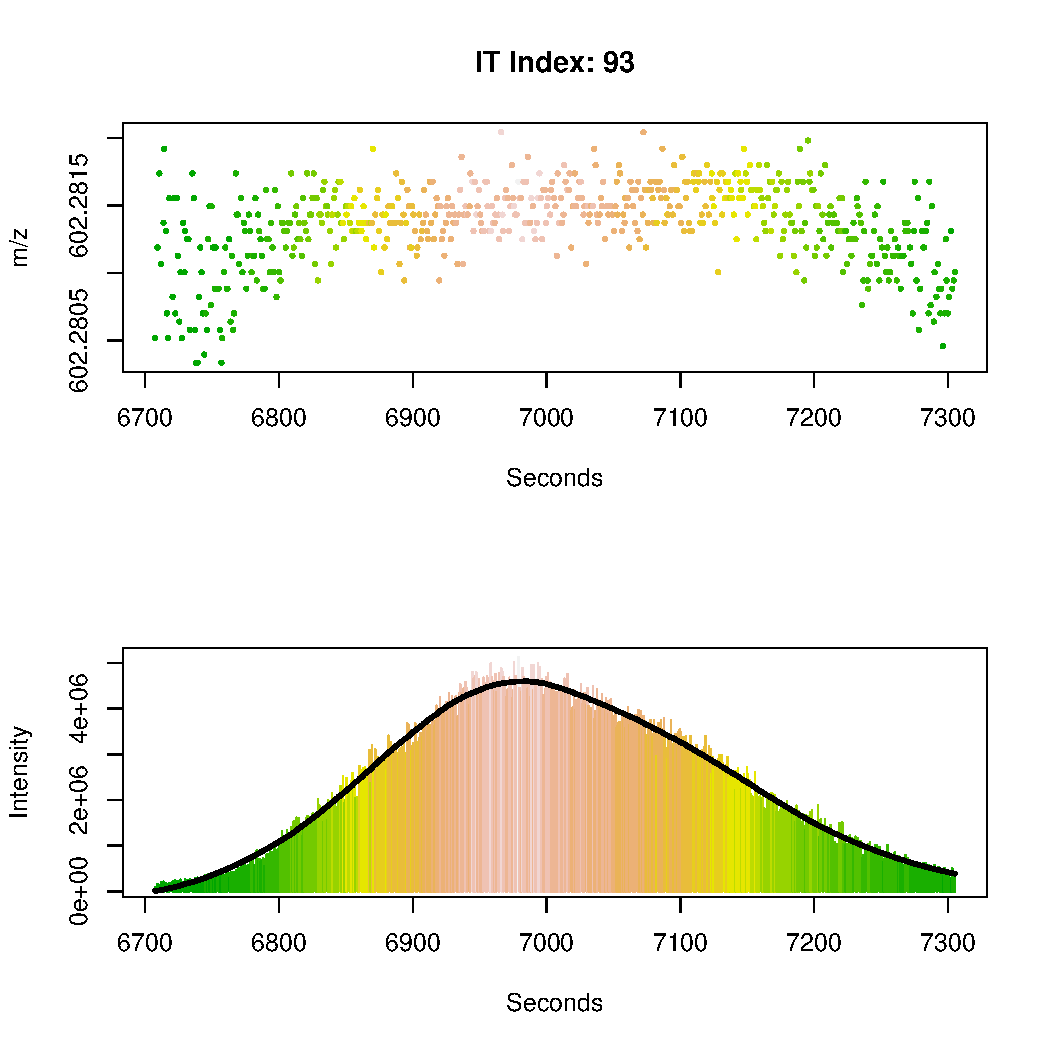
\includegraphics[width=5in,height=5in]{figs/third-pass} 

}



\end{knitrout}



The IT set generated under the RISC-driven approach is then formally evaluated based on the annotation of MOUSE. Of course, this comparison has the limitation that we chose the starting parameters cognizant of the greedy-search optimized ones. The strength of comparison would be much greater if we were blind to the formal optimization.

% latex table generated in R 3.0.2 by xtable 1.7-3 package
% Mon Mar 31 14:47:54 2014
\begin{table}[ht]
\centering
\begin{tabular}{rrrrrr}
  \hline
 & f-score(1) & IT sensitivity & IT precision & sample sensitivity & sample specificity \\ 
  \hline
Greedy Search & 0.7952 & 0.7284 & 0.8755 & 0.9334 & 0.7458 \\ 
  Visual & 0.8563 & 0.9355 & 0.7894 & 0.9610 & 0.7232 \\ 
   \hline
\end{tabular}
\caption{Greedy Search vs. Visual Optimization Results} 
\end{table}



The quick visual optimization compares well to a greedy search and happens to report less false positives at the cost of reduced sensitivity. The similarity boosts confidence in both methods' validity, despite partial evaluation dependence. 

\section{More Complicated Parameter Exploration}

 Other parameters not limited to, but including \emph{criticalValue}, \emph{ppm}, and \emph{consecMissedLim} can be optimized in Massifquant. For \emph{criticalValue} and \emph{consecMissedLim}, one parameter setting may not be a subset of another, and the tools to diagnose exact RISCs is not as precise. It should be noted that \emph{criticalValue} has been shown to vary little in performance for a wide range of values on both MOUSE and MM14 data sets (see Figures S5, S12 of Massifquant publication). It is probably one of the last parameters that should try to be optimized. An approximate RISC can be generated by evaluating the euclidean distance on the vectors [ min(m/z), max(m/z), min(time), max(time) ] between ITs of the respective parameter settings.  The function ``dset'' reports the respective indices of the approximately unique ITs contributed under different parameters.  We say the RISC is ``approximate'' because the euclidean distance sometimes identifies the same IT in two different parameter settings unique to both. \\
 
Massifquant currently hides several of the Kalman Filter model parameters (e.g. m/z estimation noise) from user manipulation that may yet still be improved. Those interested in further extending Massifquant, especially optimizing or integrating less intuitive parameters or IT filters may benefit from applying the evaluation methods contained in this section.

\begin{knitrout}
\definecolor{shadecolor}{rgb}{0.969, 0.969, 0.969}\color{fgcolor}\begin{kframe}
\begin{alltt}
\hlstd{dset} \hlkwb{<-} \hlkwa{function}\hlstd{(}\hlkwc{xs1}\hlstd{,} \hlkwc{xs2}\hlstd{,} \hlkwc{tol} \hlstd{=} \hlnum{0.001}\hlstd{) \{}
    \hlstd{it1} \hlkwb{<-} \hlstd{xs1}\hlopt{@}\hlkwc{peaks}\hlstd{[,} \hlkwd{c}\hlstd{(}\hlstr{"mzmin"}\hlstd{,} \hlstr{"mzmax"}\hlstd{,} \hlstr{"rtmin"}\hlstd{,} \hlstr{"rtmax"}\hlstd{)]}
    \hlstd{it2} \hlkwb{<-} \hlstd{xs2}\hlopt{@}\hlkwc{peaks}\hlstd{[,} \hlkwd{c}\hlstd{(}\hlstr{"mzmin"}\hlstd{,} \hlstr{"mzmax"}\hlstd{,} \hlstr{"rtmin"}\hlstd{,} \hlstr{"rtmax"}\hlstd{)]}
    \hlstd{d} \hlkwb{<-} \hlkwd{as.matrix}\hlstd{(}\hlkwd{pdist}\hlstd{(}\hlkwc{X} \hlstd{= it1,} \hlkwc{Y} \hlstd{= it2))}
    \hlstd{uniq_idx1} \hlkwb{<-} \hlkwd{sapply}\hlstd{(}\hlkwd{seq_len}\hlstd{(}\hlkwd{nrow}\hlstd{(d)),} \hlkwa{function}\hlstd{(}\hlkwc{r}\hlstd{)} \hlkwd{all}\hlstd{(d[r, ]} \hlopt{>} \hlstd{tol))}
    \hlstd{uniq_idx2} \hlkwb{<-} \hlkwd{sapply}\hlstd{(}\hlkwd{seq_len}\hlstd{(}\hlkwd{ncol}\hlstd{(d)),} \hlkwa{function}\hlstd{(}\hlkwc{c}\hlstd{)} \hlkwd{all}\hlstd{(d[, c]} \hlopt{>} \hlstd{tol))}
    \hlkwd{list}\hlstd{(}\hlkwc{uniq1} \hlstd{=} \hlkwd{which}\hlstd{(uniq_idx1),} \hlkwc{uniq2} \hlstd{=} \hlkwd{which}\hlstd{(uniq_idx2))}
\hlstd{\}}
\end{alltt}
\end{kframe}
\end{knitrout}


Now investigate the difference in unique IT produced by different settings of \emph{ppm}. Massifquant must be run two different times to capture this information.

\begin{knitrout}
\definecolor{shadecolor}{rgb}{0.969, 0.969, 0.969}\color{fgcolor}\begin{kframe}
\begin{alltt}
\hlstd{ppmthreshold} \hlkwb{<-} \hlkwd{c}\hlstd{(}\hlnum{2}\hlstd{,} \hlnum{10}\hlstd{)}
\hlcom{# run Massifquant for different ppm tolerance}
\hlstd{ppm_xs_gen} \hlkwb{<-} \hlkwa{function}\hlstd{(}\hlkwc{p}\hlstd{) \{}
    \hlkwd{xcmsSet}\hlstd{(}\hlkwc{files} \hlstd{= file_mouse,} \hlkwc{method} \hlstd{=} \hlstr{"massifquant"}\hlstd{,} \hlkwc{prefilter} \hlstd{=} \hlkwd{c}\hlstd{(}\hlnum{1}\hlstd{,} \hlnum{128750}\hlstd{),} \hlkwc{peakwidth} \hlstd{=} \hlkwd{c}\hlstd{(}\hlnum{60}\hlstd{,}
        \hlnum{100}\hlstd{),} \hlkwc{ppm} \hlstd{= p,} \hlkwc{criticalValue} \hlstd{=} \hlnum{1.5}\hlstd{,} \hlkwc{consecMissedLimit} \hlstd{=} \hlnum{2}\hlstd{,} \hlkwc{withWave} \hlstd{=} \hlnum{0}\hlstd{)}
\hlstd{\}}
\hlstd{ppm_xs} \hlkwb{<-} \hlkwd{lapply}\hlstd{(ppmthreshold, ppm_xs_gen)}
\end{alltt}
\end{kframe}
\end{knitrout}


In the case of these two ppm settings, there is absolutely no difference in the outcome (no unique indices reported.)
\begin{knitrout}
\definecolor{shadecolor}{rgb}{0.969, 0.969, 0.969}\color{fgcolor}\begin{kframe}
\begin{alltt}
\hlstd{dppm} \hlkwb{<-} \hlkwd{dset}\hlstd{(ppm_xs[[}\hlnum{1}\hlstd{]], ppm_xs[[}\hlnum{2}\hlstd{]])}
\hlstd{dppm}
\end{alltt}
\begin{verbatim}
## $uniq1
## integer(0)
## 
## $uniq2
## integer(0)
\end{verbatim}
\end{kframe}
\end{knitrout}



\subsection{Effect of Segmentation Correction}

Sometimes Massifquant does not fully track an IT, and reports the partitioned segments. The \emph{union} parameter turns on a small corrective procedure to combine contiguous m/z IT tracks. While not all segmentation-correction is favorable (e.g. combining consecutive peaks), it does help in some instances; so an analyst can quickly determine the cost or benefit with minimal effort. The code that follows illustrates how.
\begin{knitrout}
\definecolor{shadecolor}{rgb}{0.969, 0.969, 0.969}\color{fgcolor}\begin{kframe}
\begin{alltt}
\hlstd{union_status} \hlkwb{<-} \hlkwd{c}\hlstd{(}\hlnum{0}\hlstd{,} \hlnum{1}\hlstd{)}
\hlcom{# run Massifquant under different setting}
\hlstd{union_xs_gen} \hlkwb{<-} \hlkwa{function}\hlstd{(}\hlkwc{u}\hlstd{) \{}
    \hlkwd{xcmsSet}\hlstd{(}\hlkwc{files} \hlstd{= file_mouse,} \hlkwc{method} \hlstd{=} \hlstr{"massifquant"}\hlstd{,} \hlkwc{prefilter} \hlstd{=} \hlkwd{c}\hlstd{(}\hlnum{1}\hlstd{,} \hlnum{128750}\hlstd{),} \hlkwc{peakwidth} \hlstd{=} \hlkwd{c}\hlstd{(}\hlnum{60}\hlstd{,}
        \hlnum{100}\hlstd{),} \hlkwc{ppm} \hlstd{=} \hlnum{10}\hlstd{,} \hlkwc{criticalValue} \hlstd{=} \hlnum{1.5}\hlstd{,} \hlkwc{consecMissedLimit} \hlstd{=} \hlnum{2}\hlstd{,} \hlkwc{withWave} \hlstd{=} \hlnum{0}\hlstd{,} \hlkwc{unions} \hlstd{= u)}
\hlstd{\}}
\hlstd{union_xs} \hlkwb{<-} \hlkwd{lapply}\hlstd{(union_status, union_xs_gen)}
\hlcom{# RISCs determined}
\hlstd{du} \hlkwb{<-} \hlkwd{dset}\hlstd{(union_xs[[}\hlnum{1}\hlstd{]], union_xs[[}\hlnum{2}\hlstd{]])}
\hlstd{du}
\end{alltt}
\end{kframe}
\end{knitrout}


These RISC sets are easily saved to file for documentation.

\begin{knitrout}
\definecolor{shadecolor}{rgb}{0.969, 0.969, 0.969}\color{fgcolor}\begin{kframe}
\begin{alltt}
\hlkwd{plot_it_set}\hlstd{(}\hlkwc{xr} \hlstd{= data_mouse,} \hlkwc{xs} \hlstd{= union_xs[[}\hlnum{1}\hlstd{]],} \hlkwc{filename} \hlstd{=} \hlstr{"figs/no_uRISC.pdf"}\hlstd{,} \hlkwc{it_set_idx} \hlstd{= du}\hlopt{$}\hlstd{uniq1)}
\hlkwd{plot_it_set}\hlstd{(}\hlkwc{xr} \hlstd{= data_mouse,} \hlkwc{xs} \hlstd{= union_xs[[}\hlnum{2}\hlstd{]],} \hlkwc{filename} \hlstd{=} \hlstr{"figs/uRISC.pdf"}\hlstd{,} \hlkwc{it_set_idx} \hlstd{= du}\hlopt{$}\hlstd{uniq2)}
\end{alltt}
\end{kframe}
\end{knitrout}


We illustrate a useful segmentation correction example. IT index 38 has no segmentation correction, while index 65 shows the corrected version; the indices are different because they are different Massifquant runs. 
\begin{knitrout}
\definecolor{shadecolor}{rgb}{0.969, 0.969, 0.969}\color{fgcolor}\begin{kframe}
\begin{alltt}
\hlkwd{plot_it_set}\hlstd{(}\hlkwc{xr} \hlstd{= data_mouse,} \hlkwc{xs} \hlstd{= union_xs[[}\hlnum{1}\hlstd{]],} \hlkwc{it_set_idx} \hlstd{=} \hlnum{38}\hlstd{)}
\hlkwd{plot_it_set}\hlstd{(}\hlkwc{xr} \hlstd{= data_mouse,} \hlkwc{xs} \hlstd{= union_xs[[}\hlnum{2}\hlstd{]],} \hlkwc{it_set_idx} \hlstd{=} \hlnum{65}\hlstd{)}
\end{alltt}
\end{kframe}

{\centering 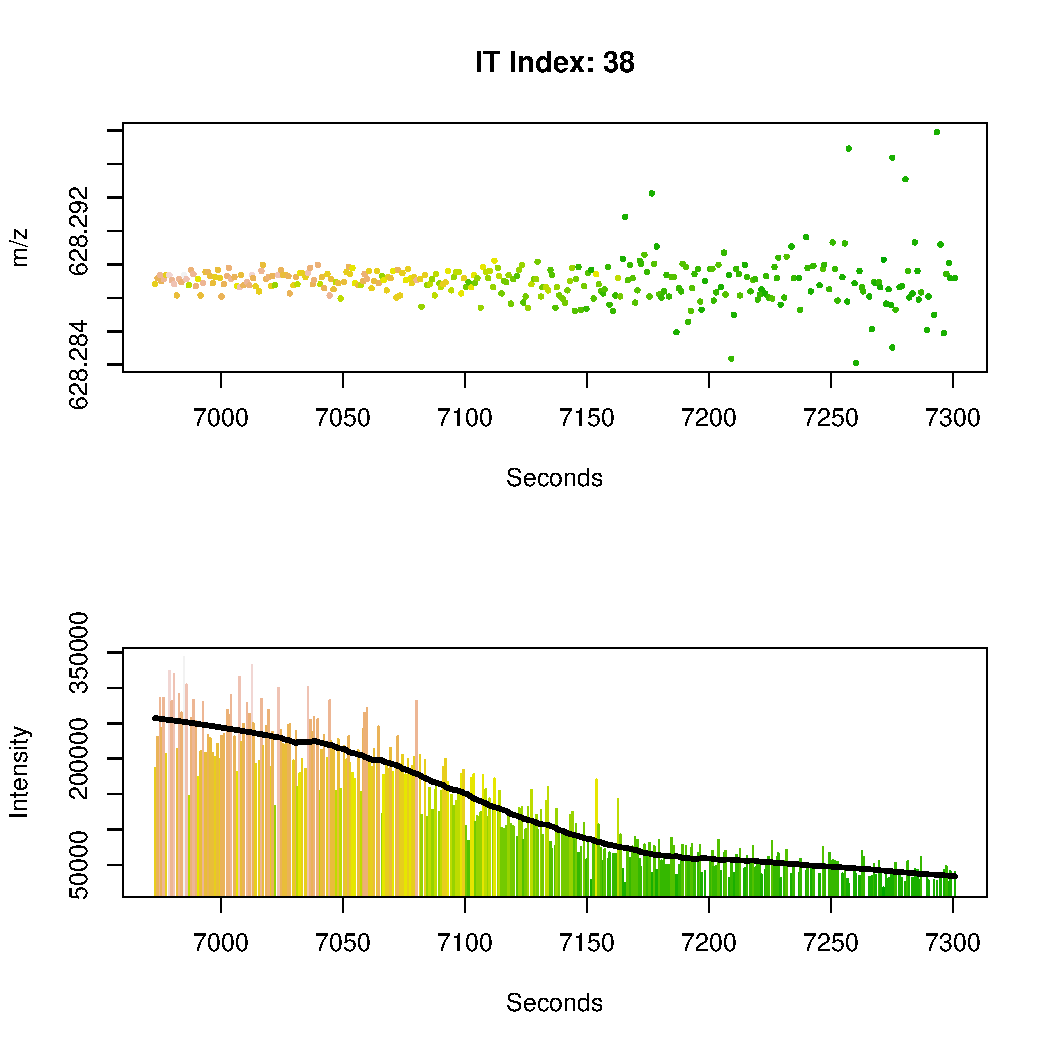
\includegraphics[width=4in,height=4in]{figs/no-seg-correction1} 
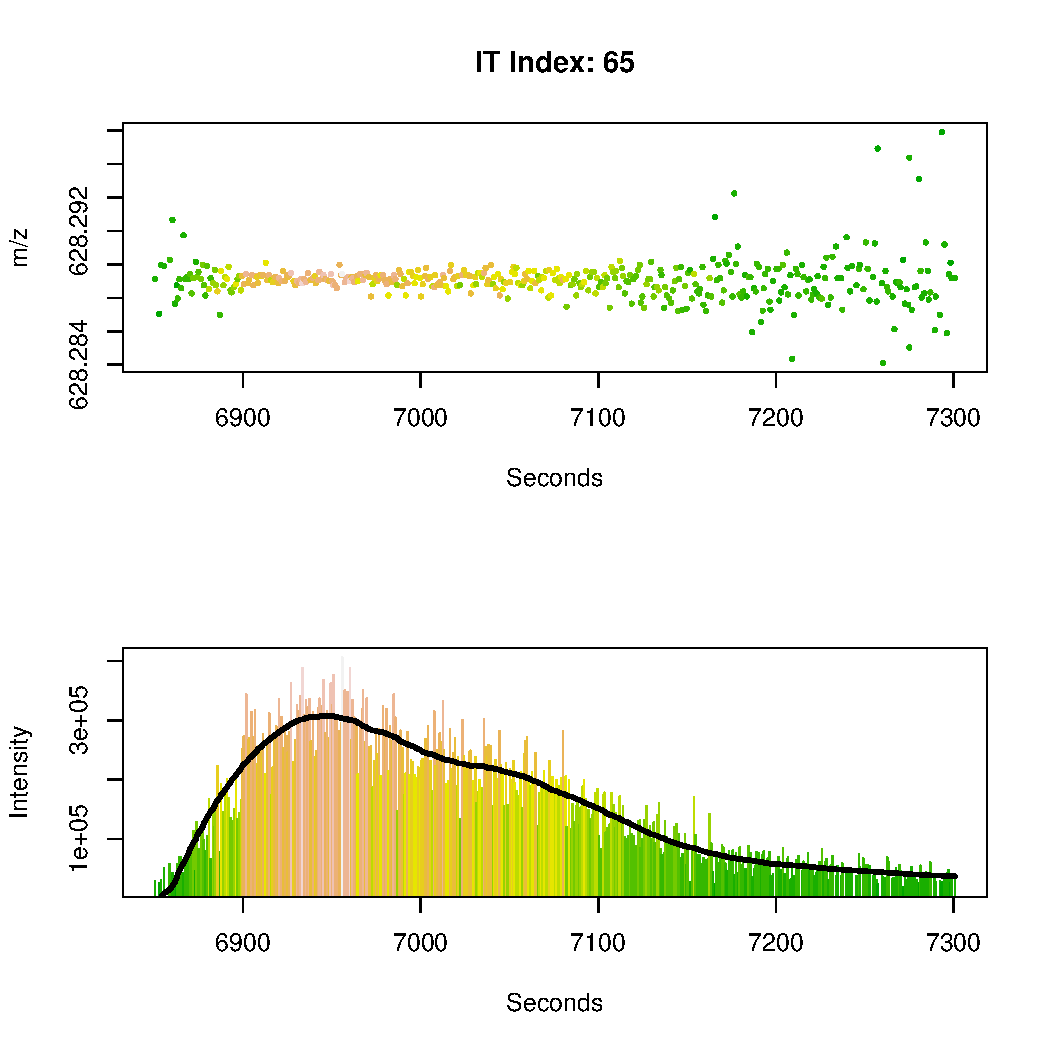
\includegraphics[width=4in,height=4in]{figs/no-seg-correction2} 

}



\end{knitrout}


\section{Conclusions}

This analysis has demonstrated the intuitive \& visual ease of sufficiently optimizing Massifquant to a particular sample without requiring a manual annotation or complex evaluation criterion.  The method is relatively quick, simple, and general enough to apply to other IT detection algorithms.

\section{Session Info}

\begin{knitrout}
\definecolor{shadecolor}{rgb}{0.969, 0.969, 0.969}\color{fgcolor}\begin{kframe}
\begin{alltt}
\hlkwd{sessionInfo}\hlstd{()}
\end{alltt}
\begin{verbatim}
## R version 3.0.2 (2013-09-25)
## Platform: x86_64-apple-darwin10.8.0 (64-bit)
## 
## locale:
## [1] en_US.UTF-8/en_US.UTF-8/en_US.UTF-8/C/en_US.UTF-8/en_US.UTF-8
## 
## attached base packages:
## [1] parallel  stats     graphics  grDevices utils     datasets  methods   base     
## 
## other attached packages:
##  [1] codetools_0.2-8    pdist_1.2          signal_0.7-3       MASS_7.3-30       
##  [5] xtable_1.7-3       xcms_1.39.5        Biobase_2.22.0     BiocGenerics_0.8.0
##  [9] mzR_1.8.1.1        Rcpp_0.11.0        knitr_1.5         
## 
## loaded via a namespace (and not attached):
## [1] evaluate_0.5.1 formatR_0.10   highr_0.3      stringr_0.6.2  tools_3.0.2
\end{verbatim}
\end{kframe}
\end{knitrout}


\end{document}
